% !TEX root=/home/tavant/these/manuscript/src/manuscript.tex

% \FloatBarrier

    
    \section{Maximum electron temperature in experiments}
    
    
    In \citet{raitses2006}, the authors compare the maximum of the axial profile of the electron temperature $\hat{\Te}$ measured in a \ac{HET} with two different wall materials\string: one with a very low emissivity (carbon velvet material), the other is the conventional \ac{BN} ceramic.
    \Cref{fig-raiteses2006} reproduces the results obtained in \citet{raitses2006}.

    \begin{figure}[hbt]
      \centering
      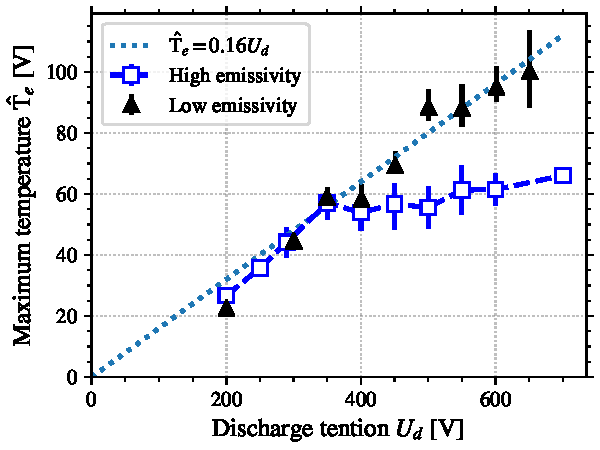
\includegraphics[width=\defaultwidth]{Raiteses_remaked.pdf}
      \caption{ The dependence of the maximum electron temperature on the discharge  voltage for a conventional thruster with high-SEE \acs{BN} channel walls and the segmented thruster with low-SEE floating segmented electrodes made of carbon velvet material. Reproducibility of measurements is shown by error bars. Adapted from \citet[Fig. 3]{raitses2006} }
      \label{fig-raiteses2006}
    \end{figure}

    They observed that with the \ac{BN} ceramic the values of $\hat{\Te}$ reach a plateau.
    The value of the plateau is $\hat{\Te}^1 = 55 \pm 6\,\volt$, the error corresponds to reproducibility of the measurements.
    In contrast the results with the low emissivity material do not present such behavior, but instead the electron temperature $\hat{\Te}$ keeps increasing linearly with the discharge voltage.
    
    The saturation of the temperature is expected to be due to the \ac{SCL} regime, which increases the electron power losses.
    Hence, we expect that the plateau to be the related to $\Te^1$ the maximum electron temperature for the first root S1 to exist.
    For the \ac{BN} ceramic we have $\crover \simeq 35\,\volt$ \citep{smirnov2004}, hence using $\gamma=1.36$ we have $\Te^1 = 45\,\volt$.
    This value is lower than $\hat{\Te}^1$ observed experimentally, but the agreement is significantly better than with the isothermal sheath model prediction\string:
    \begin{equation} \label{eq-Temaxisothermal}
      \Te^1_{\rm , isothermal} \simeq \frac{\crover}{2} \simeq 17.5 \,\volt.
    \end{equation}
    
    In order to assess the discrepancy between  $\Te^1$ and $\hat{\Te}^1$, we need to know the polytropic index observed experimentally.
    In addition, several phenomena are neglected in the \ac{2D} \ac{PIC} simulation of the sheath model, as the magnetic mirror and the channel curvature \citep{heron2013,dominguez-vazquez2018}.
    
    % One possible explanation of the difference between the PIC is the anisotropy of the electrons.
    % Indeed, the probe measurements measure the average electron temperature, in contrast with the sheath theory which suppose that the electrons are isotropic.
    